\documentclass{article}
\usepackage{graphicx}
\usepackage{listings}
\usepackage{geometry} % Required for customizing margins
\geometry{margin=1in} % Sets 1-inch margins on all sides

\begin{document}

\title{Fundamentals of Communications Computer Assignment 1}
\author{Jacob C. Vaught}
\date{September 2nd, 2023}
\maketitle
\section*{Problem \#1}

The waveform \( x(t) = A \sin(2\pi f_c t) \cos(2\pi f_i t) \) is a product of two sinusoidal functions. The parameters \( A \), \( f_c \), and \( f_i \) represent the amplitude, frequency of the sine wave, and frequency of the cosine wave, respectively.
\subsection*{Theoretical Explanation}
To plot this function for two full cycles, the period of the function is needed first. The period \( T \) of a sine or cosine function \( \sin(2\pi f t) \) or \( \cos(2\pi f t) \) is \( T = \frac{1}{f} \).
\newline
Here, \( f_c = 32 \) and \( f_i = 2 \), so their periods are \( \frac{1}{32} \) and \( \frac{1}{2} \), respectively. To find the period of the combined function \( x(t) \), look for the least common multiple (LCM) of the individual periods. 
\subsection*{Results}
\begin{figure}[!h]
\centering
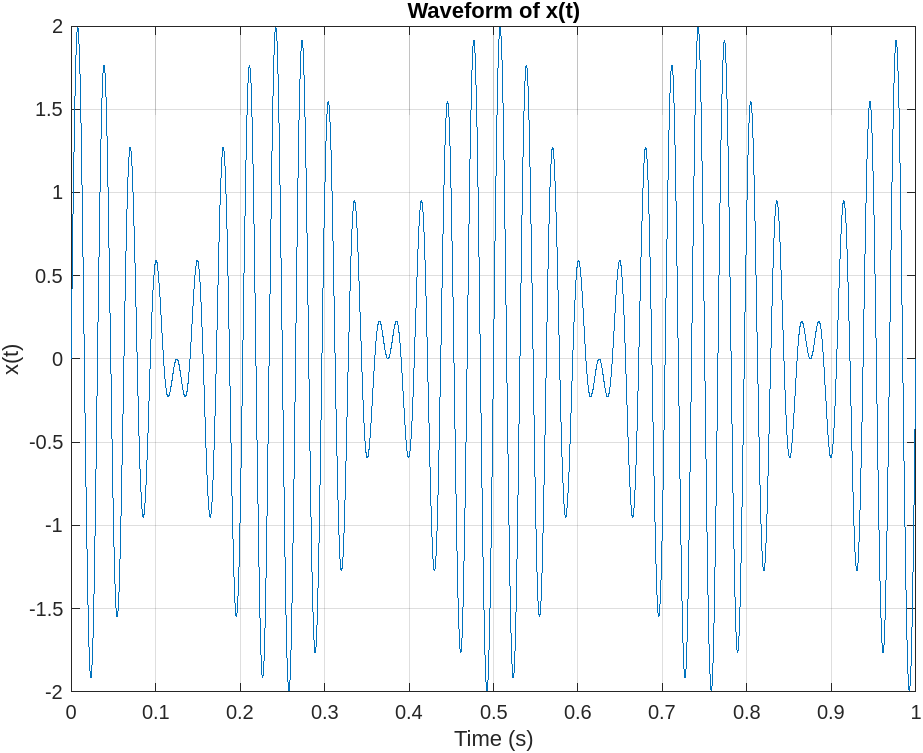
\includegraphics[width=0.8\textwidth]{Figure_HW1_p1.png}
\caption{Waveform of \( x(t) \)}
\end{figure}
\subsection*{Conclusion}
To determine if \( x(t) \) is periodic, look at the plot. A function is periodic if it repeats its values in regular intervals or periods. From the plot, the function is indeed periodic.
\newline \newline
For a function \( x(t) \) to be periodic, there must exist a \( T > 0 \) such that \( x(t + T) = x(t) \, \forall t \). In this case, the function does repeat its form. To find its period, look at the least common multiple (LCM) of the periods of the individual sine and cosine components. The period of the sine wave is \( T_c = \frac{1}{f_c} = \frac{1}{32} \) and the period of the cosine wave is \( T_i = \frac{1}{f_i} = \frac{1}{2} \). Therefore, \( x(t) \) is periodic with a period of approximately 0.5 seconds.
\subsection*{MATLAB Code}
\begin{verbatim}
A = 2;
fc = 32;
fi = 2;

t = linspace(0, 2 * (1/fi), 10000); % 10000 points for smoothness
x_t = A * sin(2 * pi * fc * t) .* cos(2 * pi * fi * t);

figure;
plot(t, x_t);
xlabel('Time (s)');
ylabel('x(t)');
title('Waveform of x(t)');
grid on;
\end{verbatim}

\newpage
\section*{Problem \#2}
\subsection*{Theoretical Background}
In wireless communications, multipath propagation occurs when a transmitted signal encounters multiple paths before reaching the receiver. Each path can have a different length, phase, and attenuation, causing multiple copies of the signal to arrive at the receiver at different times and amplitudes. 
\newline \newline
The frequency response \(H(f)\) of a multipath channel is mathematically represented by the equation:
\[
H(f) = \sum_{n=0}^{N-1} h_n e^{-j 2 \pi f t_n}
\]
\newline
where \(h_n\) are the gains and \(t_n\) are the time delays of each path. This equation serves as the basis for our MATLAB code. Specifically, we use an array \( h = [0.1, 0.1, 1, 1.1, -0.2] \) to represent the gains \(h_n\) and an array \( t = [0, 0.1e^{-6}, 0.7e^{-6}, 1.1e^{-6}, 3e^{-6}] \) to represent the time delays \(t_n\).
In the code, we first define these constants and then loop through a frequency range from 1845 MHz to 1855 MHz. For each frequency \( f \), we calculate \( H(f) \) using the equation above. This is computed in MATLAB using the `exp` function for the complex exponential and the `sum` function to perform the summation.

\subsection*{Results}
The frequency response of the multipath communication channel was simulated and plotted over the frequency range of 1845 MHz to 1855 MHz. The magnitude of the frequency response, \( |H(f)| \), varies significantly across the given frequency range.
\begin{figure}[h]
  \centering
  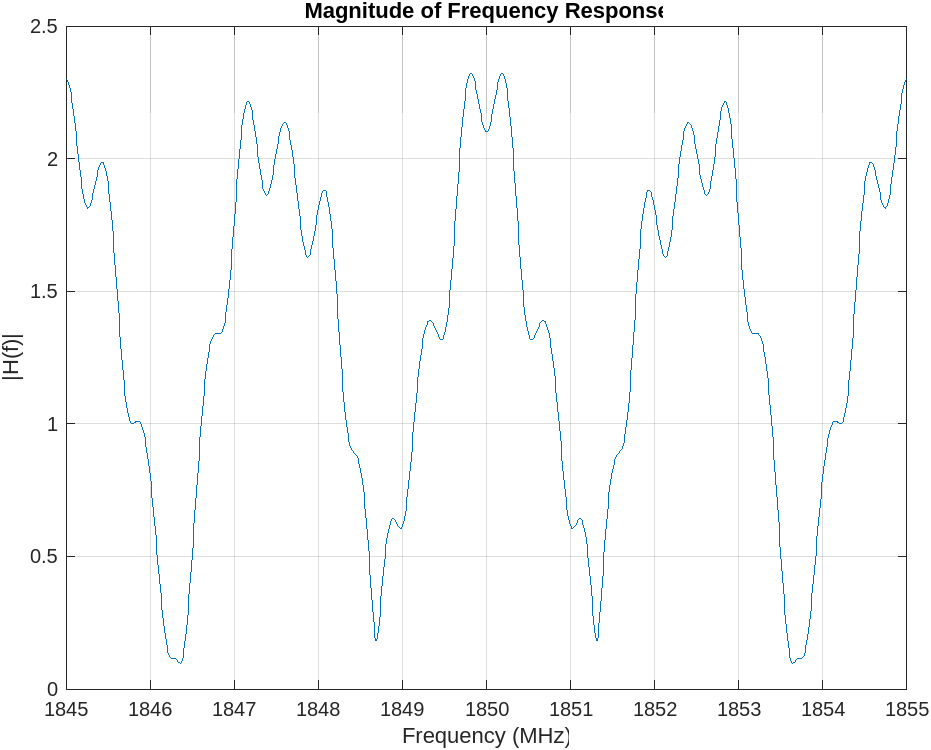
\includegraphics[width=0.8\textwidth]{Figure_HW1_p2.png}
  \caption{Magnitude of Frequency Response}
\end{figure}
\newline 
Fading frequencies were identified, occurring at 1851.31, 1846.36, 1848.69, \& 1853.64 MHz.

\subsection*{Discussion}

The plot indicates a complex behavior of the multipath communication channel across the given frequency range. Peaks in the frequency response plot suggest frequencies at which the channel performs well, while troughs or low points suggest frequencies where the signal would fade. Specifically, frequencies near 1851.31, 1846.36, 1848.69, \& 1853.64 MHz appear to be particularly prone to fading.

\subsection*{MATLAB Code}
\begin{verbatim}
% Define constants
h = [0.1, 0.1, 1, 1.1, -0.2];
t = [0, 0.1e-6, 0.7e-6, 1.1e-6, 3e-6];
frequencies = linspace(1845e6, 1855e6, 1000);

% Compute the frequency response
H_f = zeros(1, length(frequencies));

for k = 1:length(frequencies)
    f = frequencies(k);
    H_f(k) = sum(h .* exp(-j * 2 * pi * f * t));
end

% Calculate the magnitude of frequency response
magnitude_H_f = abs(H_f);

% Plot the magnitude of frequency response
figure;
plot(frequencies/1e6, magnitude_H_f);
xlabel('Frequency (MHz)');
ylabel('|H(f)|');
title('Magnitude of Frequency Response');
grid on;
\end{verbatim}

\end{document}